% Supplementary materials for: Estimating Cuba's 2021--2026 population collapse
\documentclass[11pt,a4paper]{article}

\usepackage[margin=2.2cm]{geometry}
\usepackage{times}
\usepackage{amsmath,amssymb}
\usepackage{graphicx}
\usepackage{booktabs}
\usepackage{hyperref}
\usepackage{setspace}
\usepackage{caption}
\usepackage{natbib}
\setstretch{1.12}
\captionsetup[figure]{font=small,labelfont=bf,skip=6pt}

\graphicspath{{../../../figures/}}

\title{Supplementary materials:\\
Estimating Cuba's 2021--2026 population collapse}
\author{Yasset P\'erez-Riverol}
\date{Preprint supplement · 31 July 2026}

\begin{document}
\maketitle

\noindent These materials accompany the main preprint.
Preferred public estimates remain Model~D; Model~E is provisional and is not used for headline claims~\citep{repo,modele_supp}.

\section{Life expectancy series}
Official life expectancy at birth peaked in 2011--13 (78.5 years) and fell to 77.7 in 2018--20, before the worst of the present crisis (Figure~\ref{fig:le}).
An independent 2021 estimate places it near 71 years~\citep{albizu2023,bronnum2023}.
Life expectancy re-expresses the same mortality shock rather than providing independent corroboration; its magnitude (about 6.5 years in a single year in the independent path) is exceptional for peacetime and large even relative to COVID-era losses documented internationally~\citep{aburto2022,msemburi2023}.
Translated to years of life lost, crude excess of $\sim$153{,}000 deaths in 2020--2025 implies more than one million person-years lost, concentrated among the elderly.

\begin{figure}[!htbp]
\centering
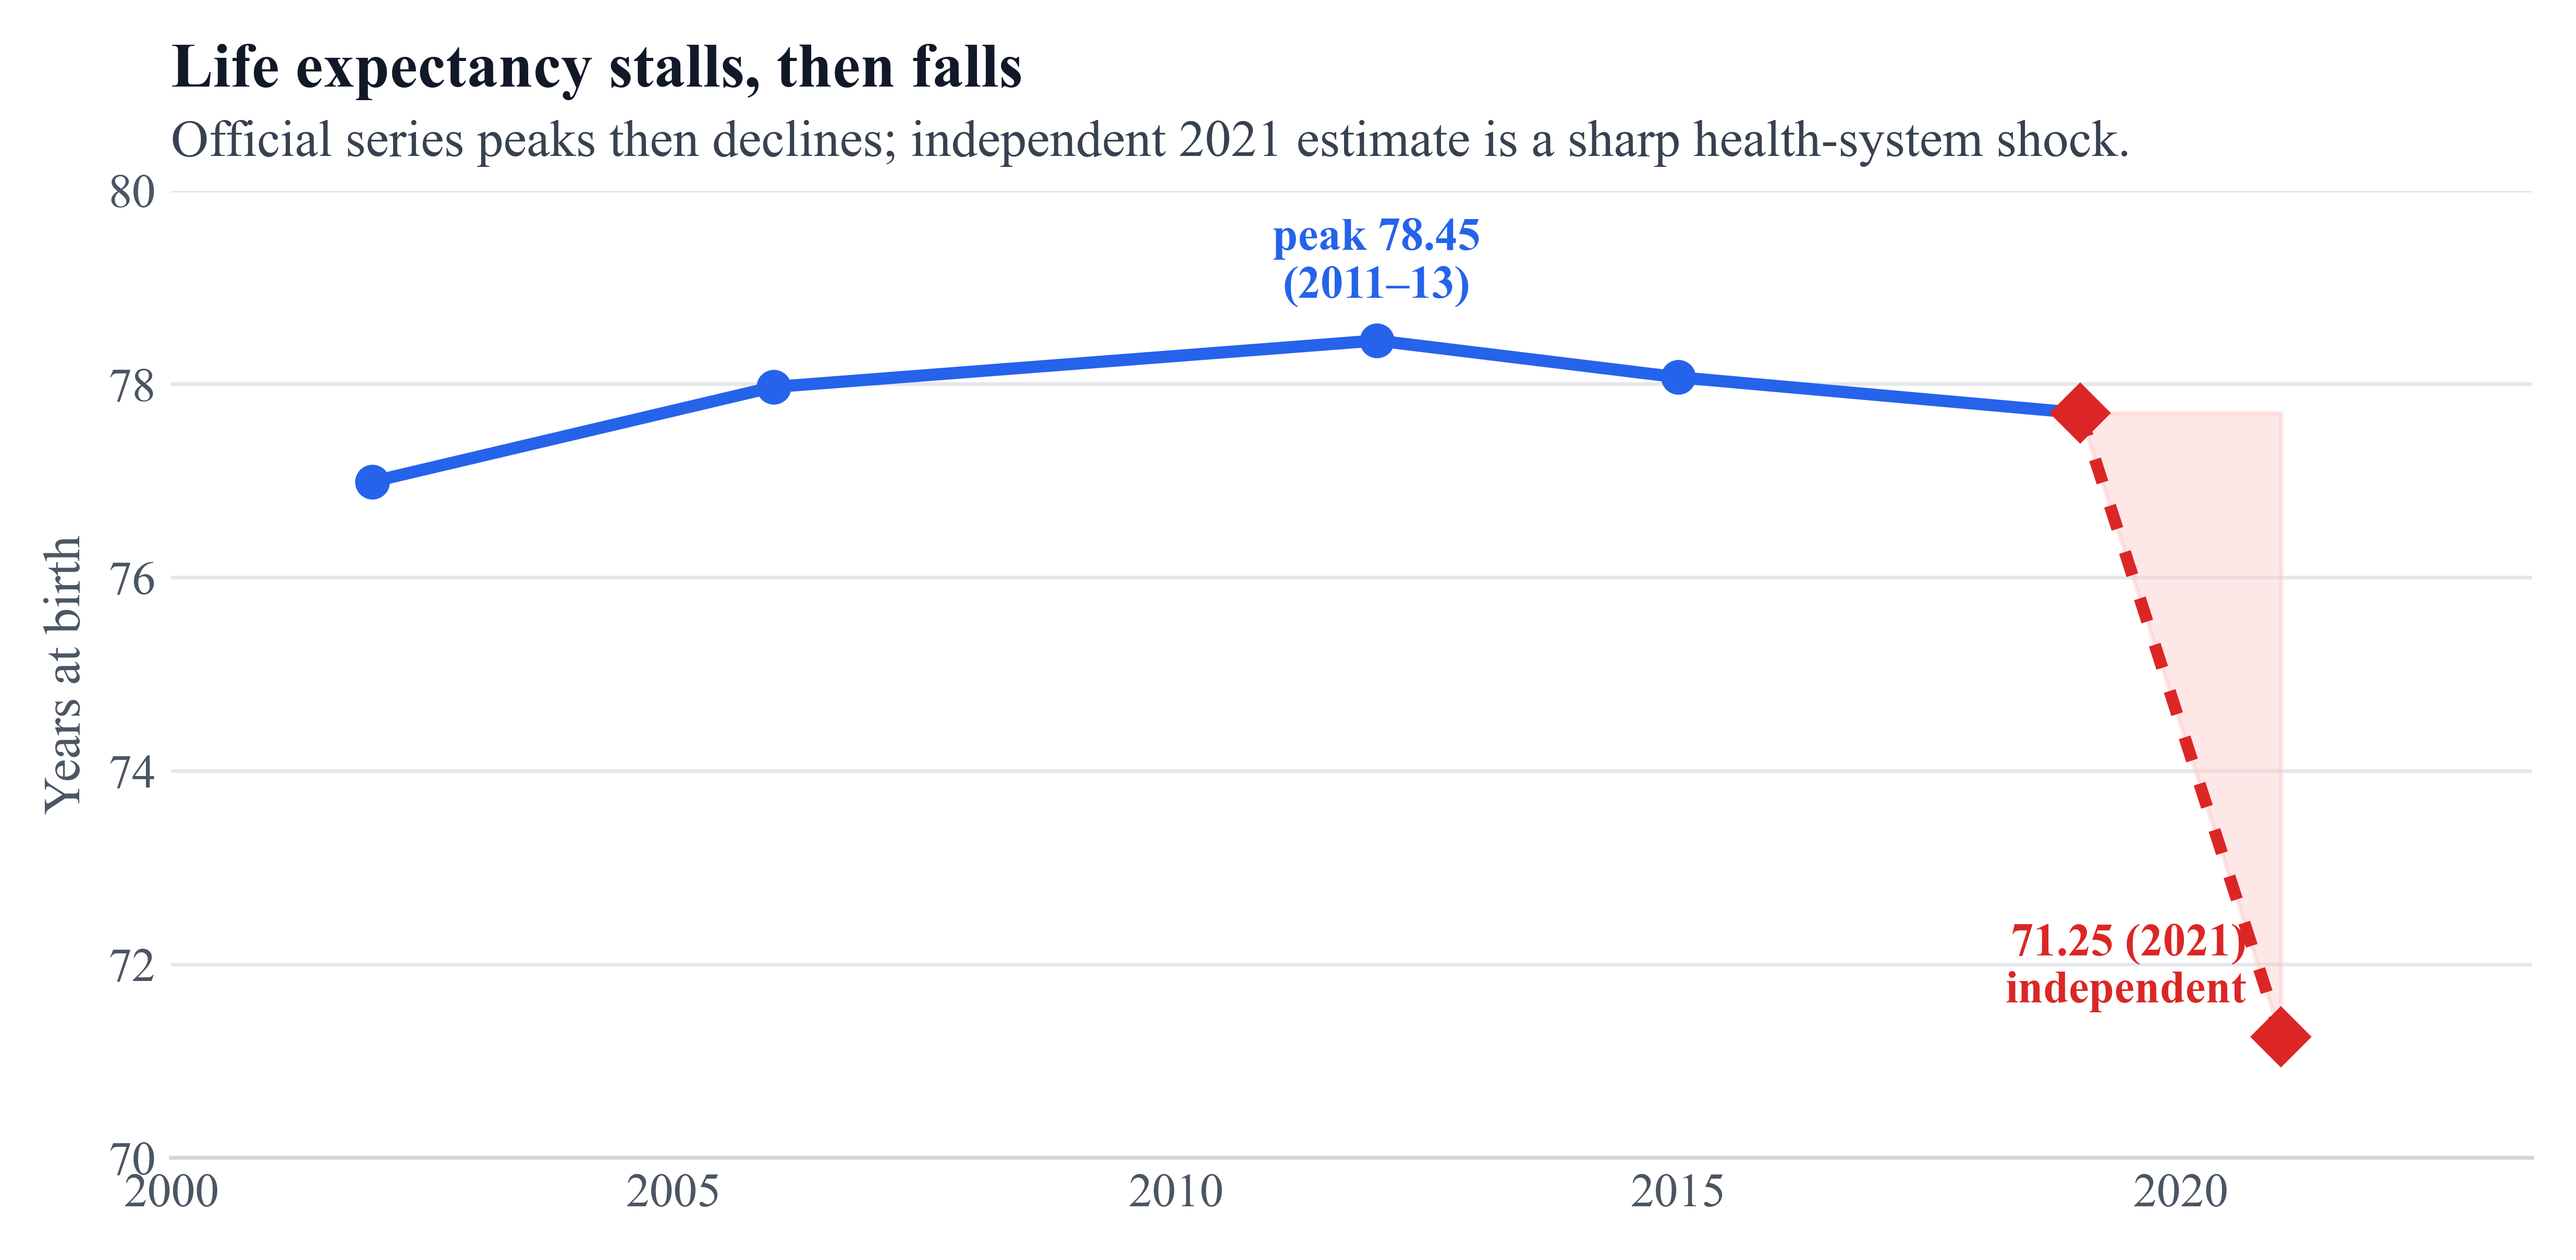
\includegraphics[width=0.85\linewidth]{f5_esperanza.png}
\caption{Life expectancy at birth: official triennial series and independent 2021 estimate.}
\label{fig:le}
\end{figure}

\section{Provincial intensity of exit}
Emptying is national but unequal (Figure~\ref{fig:prov}).
Havana leads at net emigration of \textbf{$-$33 per 1{,}000} in 2025; western and central provinces empty faster than the east, yet no province loses less than about 2\% of its people per year~\citep{onei_2025}.

\begin{figure}[!htbp]
\centering
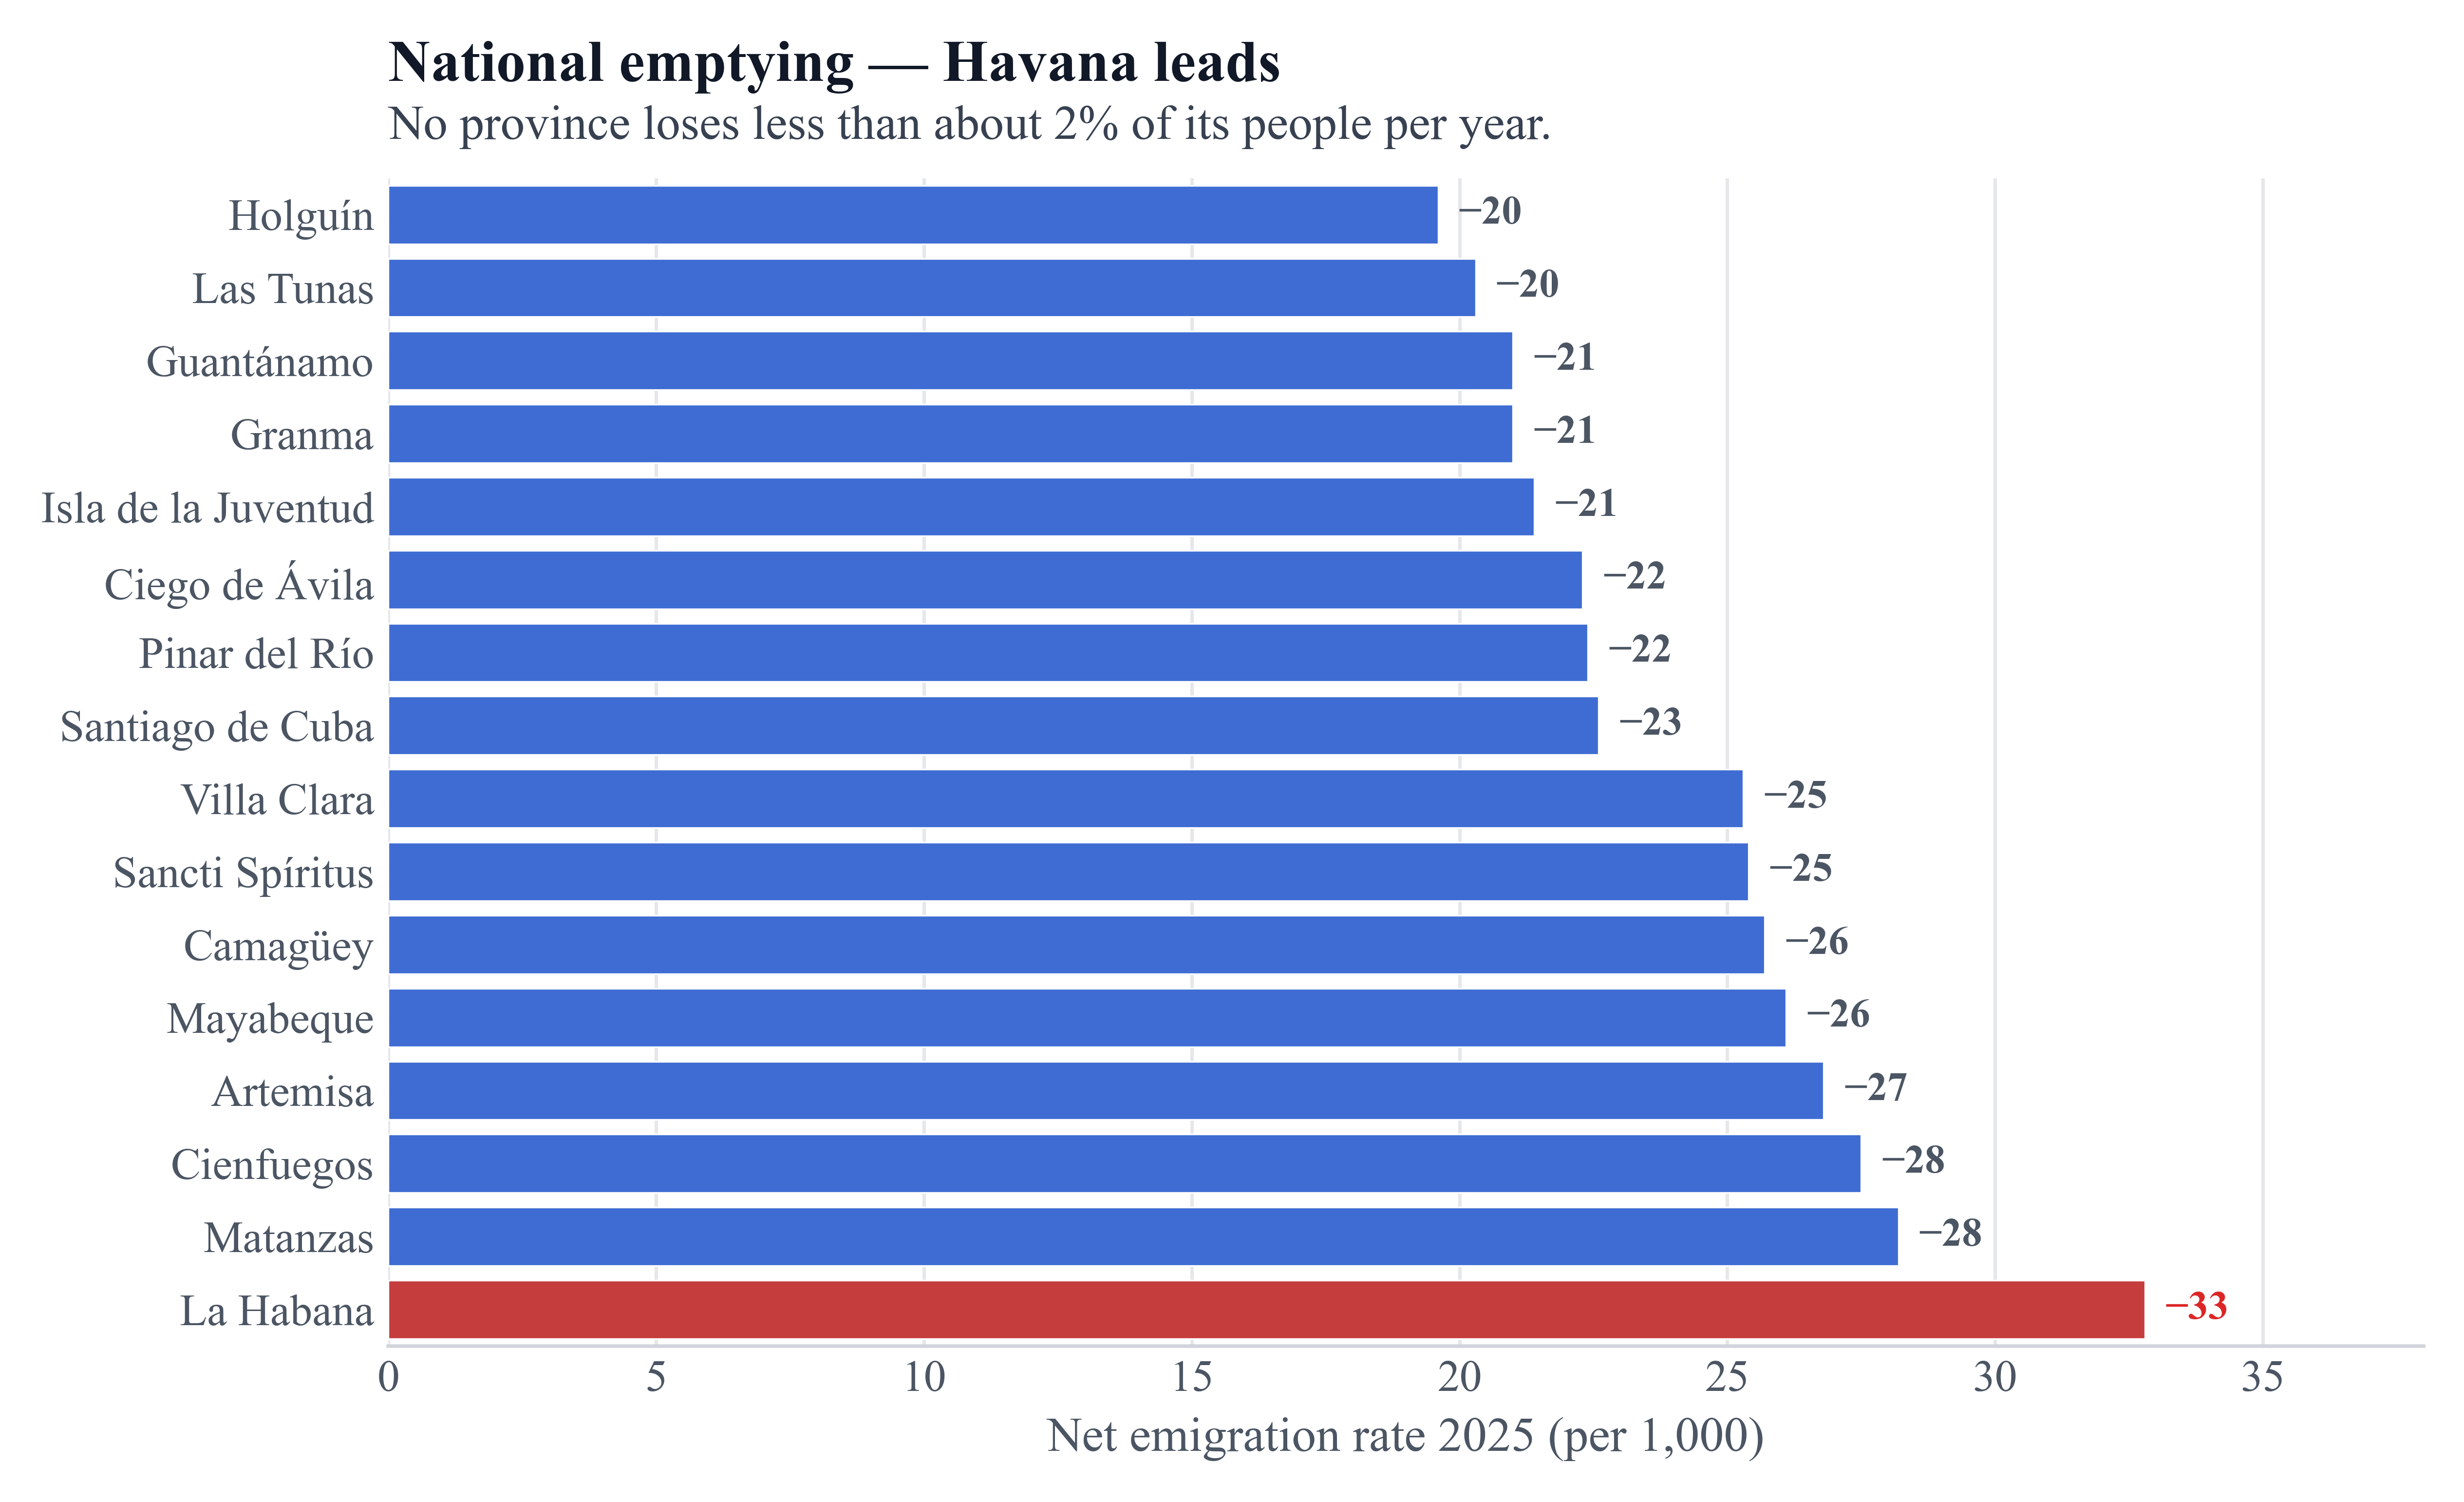
\includegraphics[width=0.9\linewidth]{f11_provincias.png}
\caption{Net emigration rate by province, 2025.}
\label{fig:prov}
\end{figure}

\section{Model E: vital reconstruction (provisional)}
As a companion path, Model~E reconstructs \emph{true} deaths and births from a yearly health-system deterioration score $S_t$ built from ageing, health-system decadence, and documented official underreporting (including COVID cause-attribution misuse as an integrity feature, not as a $\times N$ multiplier on all deaths).
The approach follows the spirit of excess-mortality reconstruction under incomplete registration~\citep{karlinsky2021,msemburi2023,kishore2018}, but uses a Cuban-specific deterioration score rather than a pandemic-only counterfactual.

Ageing enters an expected-death schedule; decadence raises an uplift $f(S_t)$; births stay near the register with crisis fertility and selective exit.
Closing the identity $P^*=P^*_{\mathrm{start}}+\sum(B^*-D^*-M^*)$ with a Model~D-like migration bridge yields median end-2025 population about \textbf{8.96~million} (loss 2.13~million, 19.2\% on the corrected base; migration share $\sim$88\%).
Figure~\ref{fig:hsds} shows $S_t$ and reconstructed versus registered vitals; Figure~\ref{fig:modele} places E beside A--D.

Preferred public claims remain Model~D until an adversarial gate promotes E.
Model~E lands in the same loss band as D and raises the natural-decrease share only modestly ($\sim$12\% versus $\sim$9\% under D), so it does not yet displace D for public claims~\citep{repo}.

\begin{figure}[!htbp]
\centering
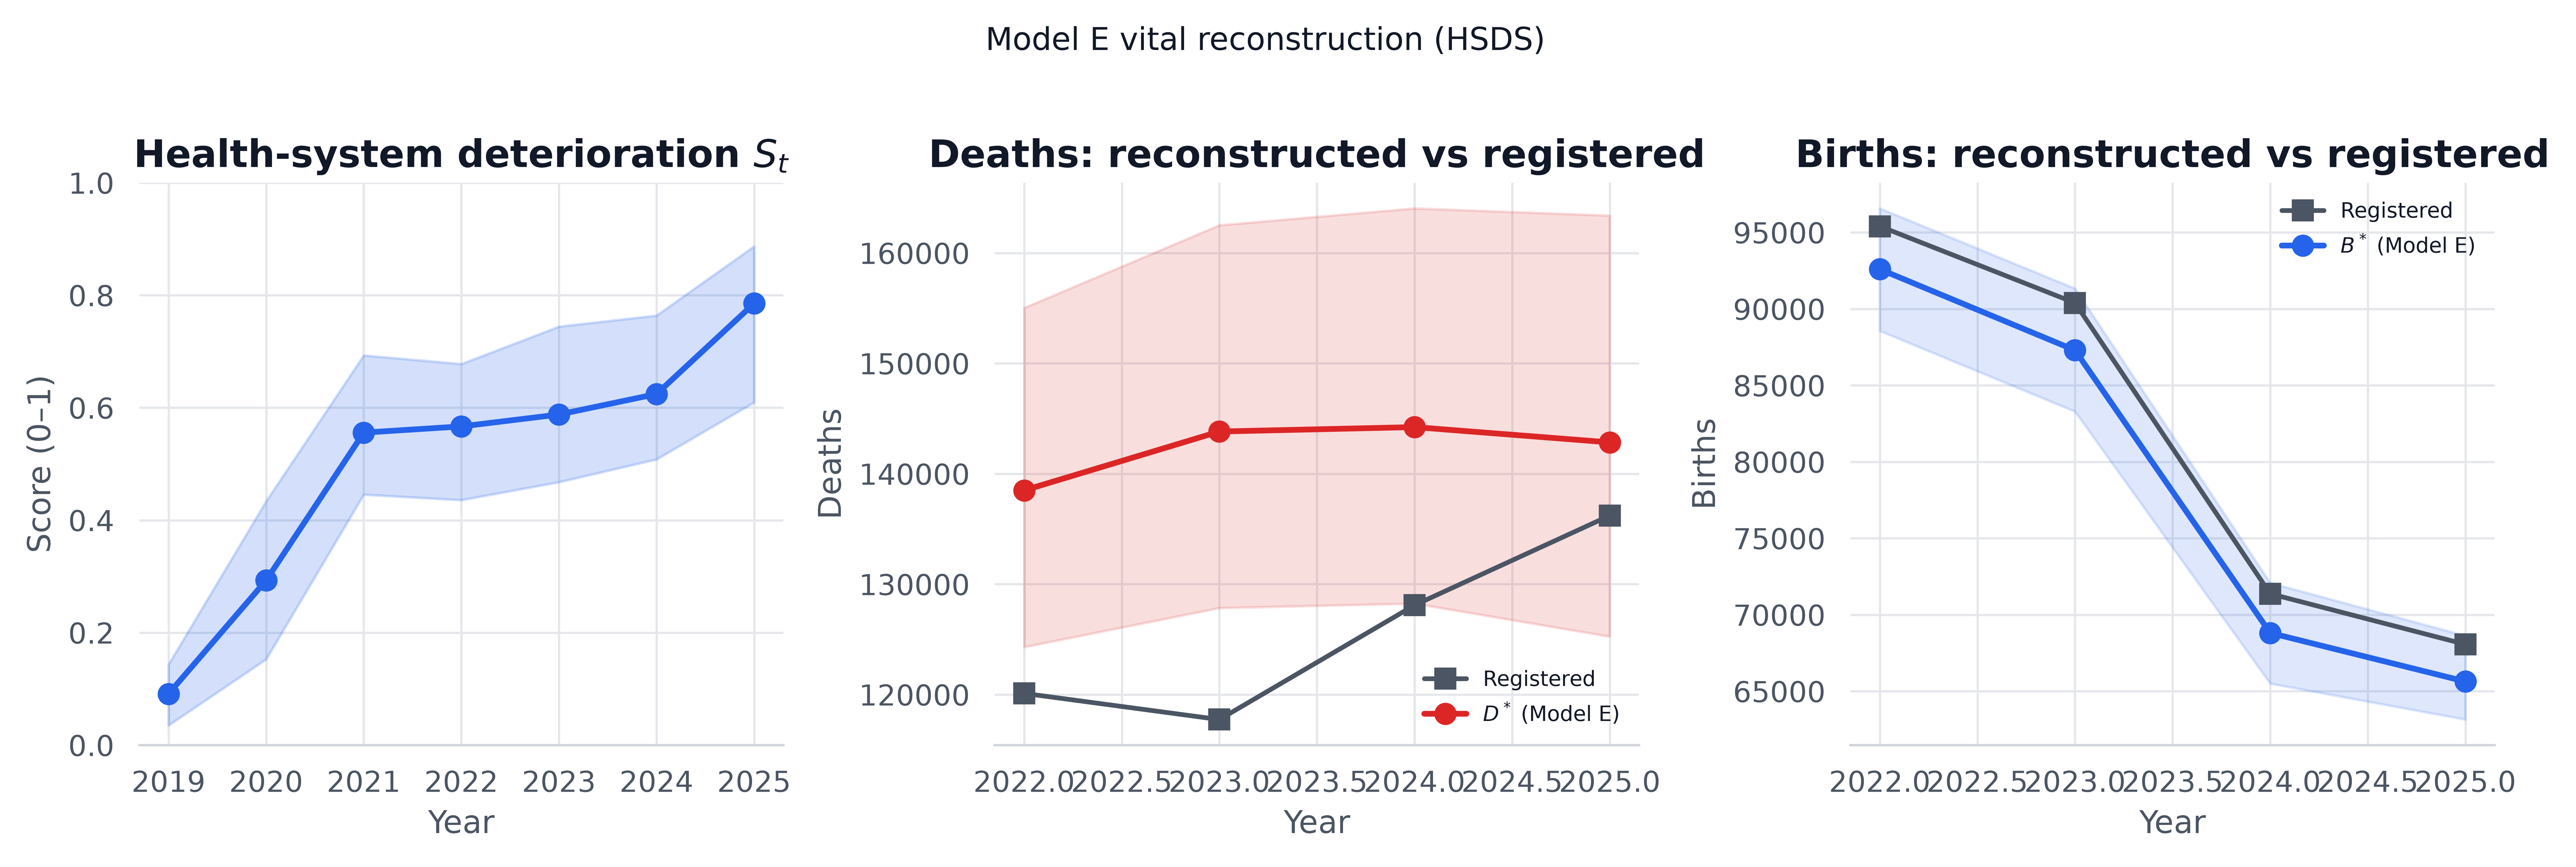
\includegraphics[width=\linewidth]{f12_hsds_vitals.png}
\caption{Health-system deterioration score $S_t$ and Model~E reconstructed deaths/births versus registered series (2022--2025).}
\label{fig:hsds}
\end{figure}

\begin{figure}[!htbp]
\centering
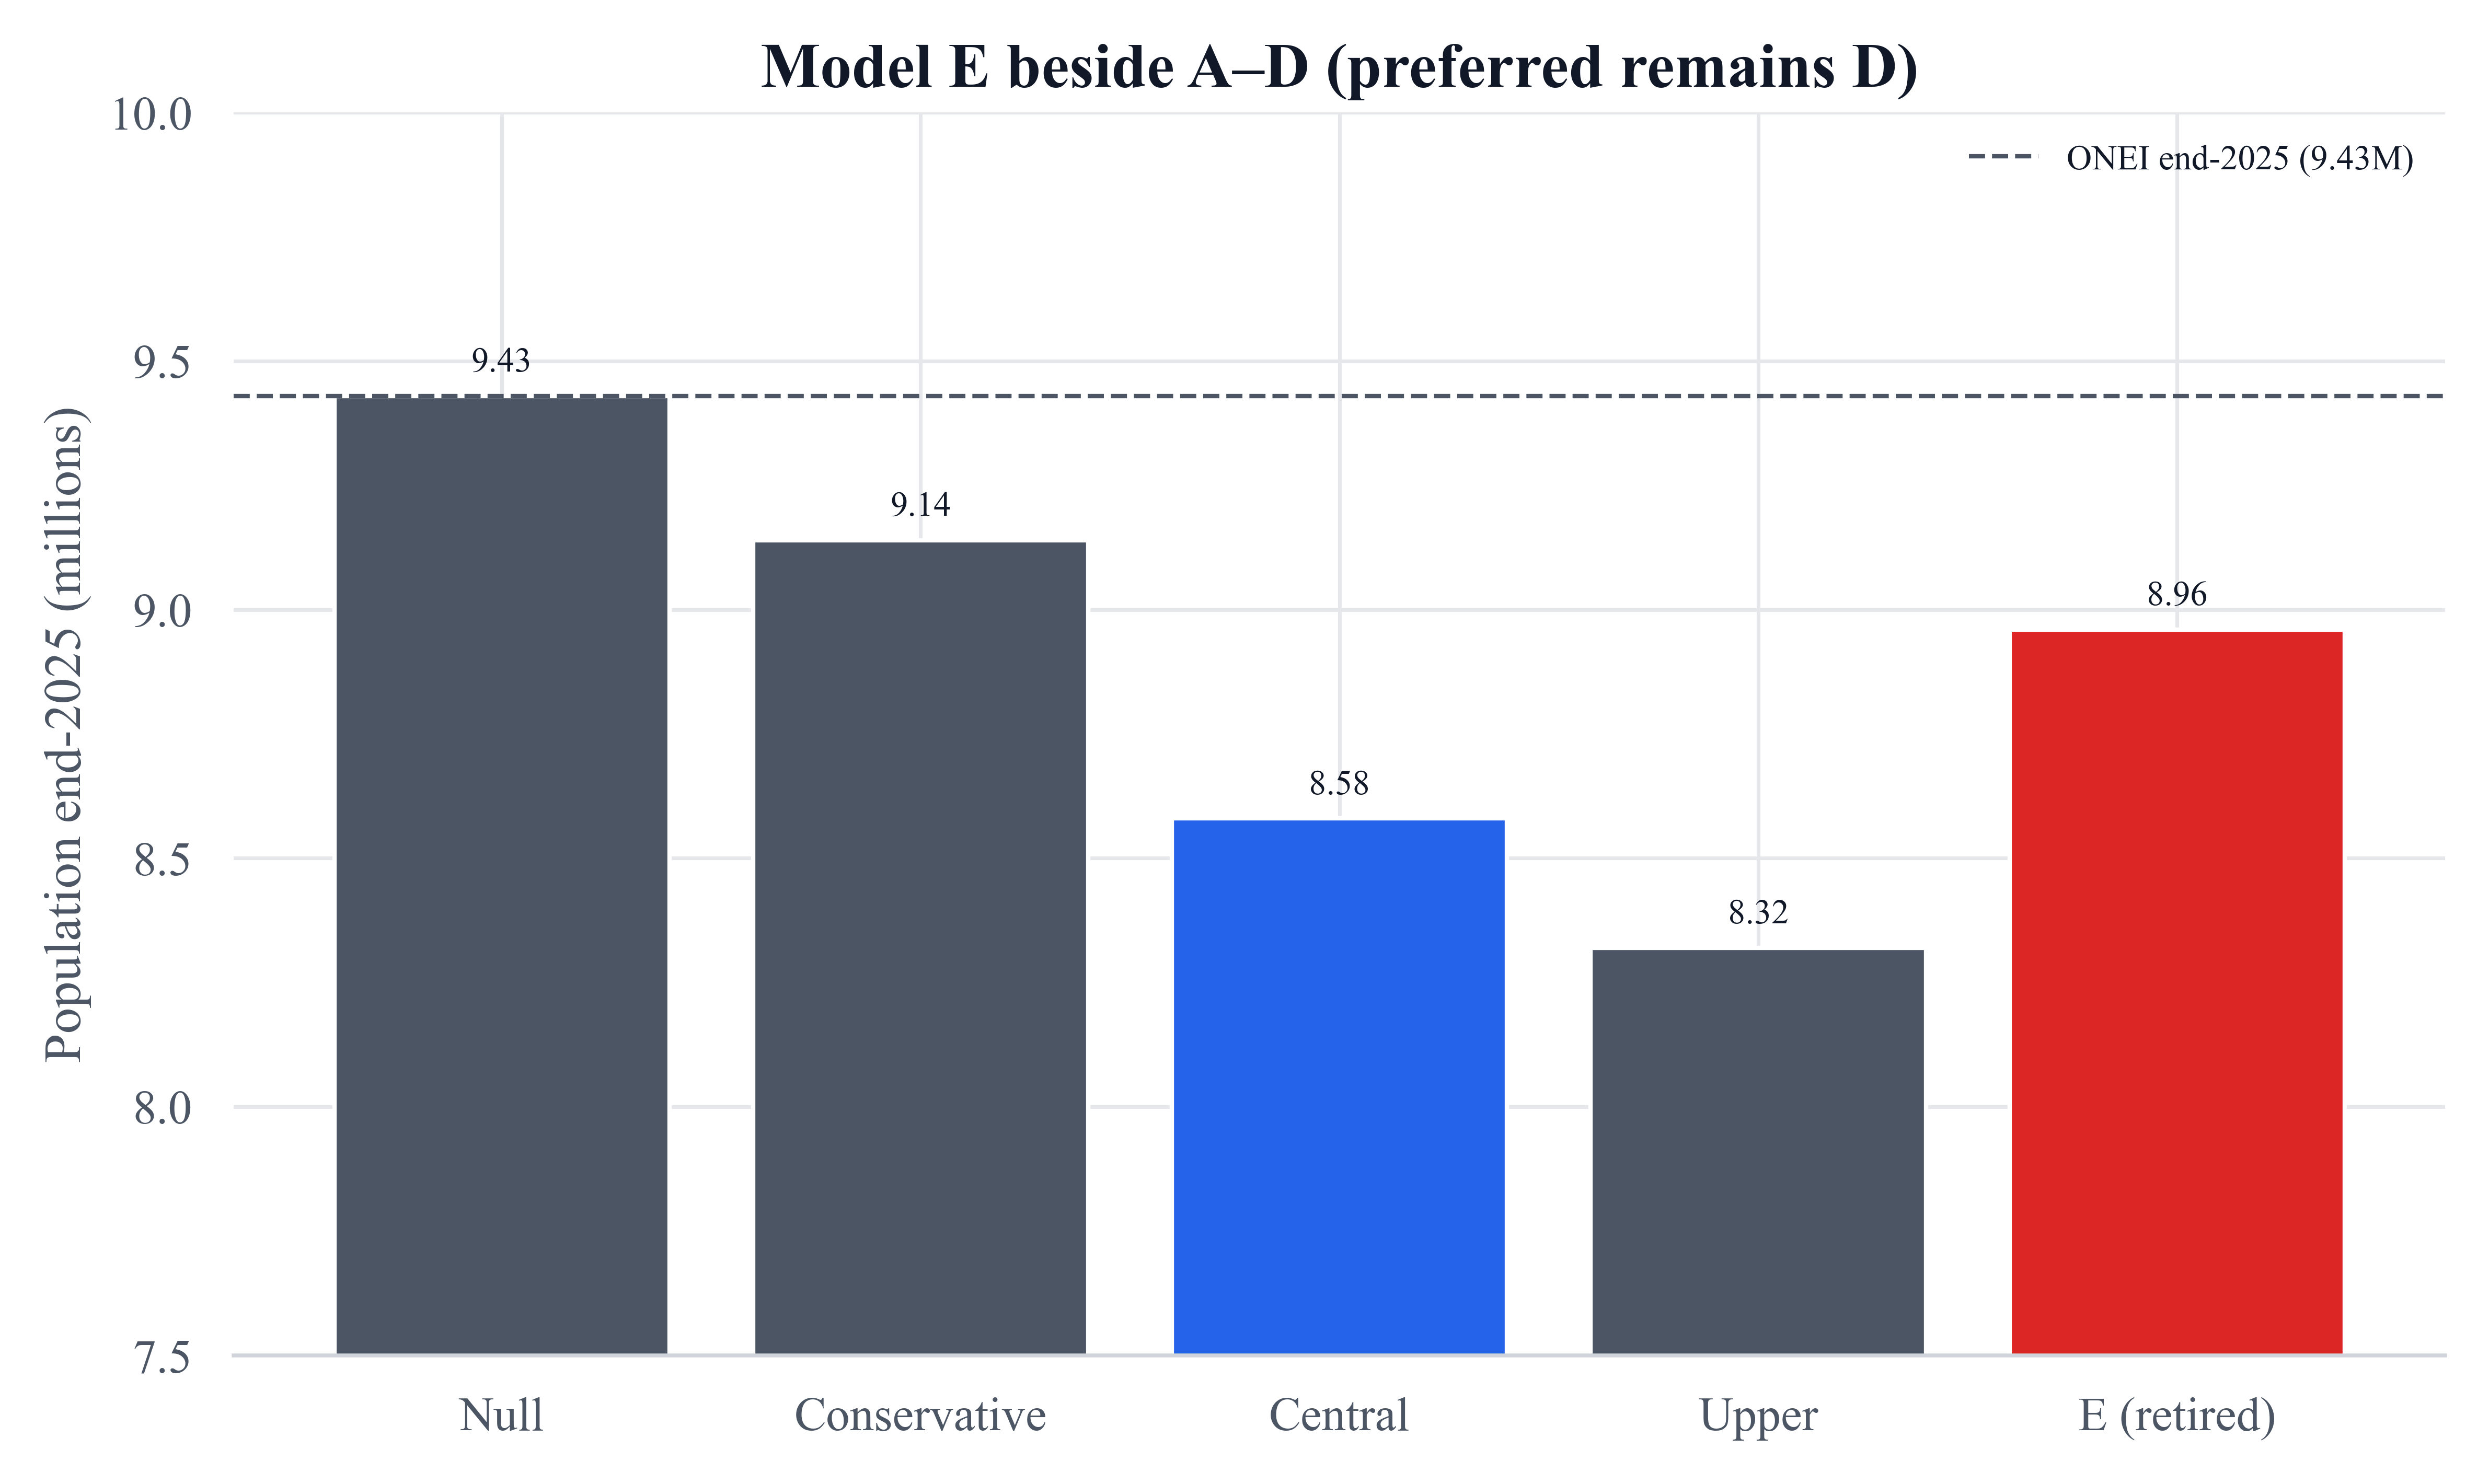
\includegraphics[width=0.72\linewidth]{f13_model_e_population.png}
\caption{End-2025 population medians for Models A--E. Preferred public model remains D (blue); E (red) is provisional.}
\label{fig:modele}
\end{figure}

\begin{table}[ht]
\centering
\caption{Models A--E medians (end-2025). Model~E is provisional and reported only here.}
\label{tab:modelsE}
\begin{tabular}{llrrr}
\toprule
Model & Main assumption & Loss (M) & \% & Pop.\ (M) \\
\midrule
A · conservative & ONEI-anchored & 1.80 & 16.4 & 9.16 \\
B · crisis-adjusted & under-reg.\ + independent migration & 2.19 & 20.4 & 8.57 \\
C · worst case & analog upper bound & 2.41 & 22.6 & 8.26 \\
D · sentinel (preferred) & IMR sentinel + triangulation & 2.21 & 20.5 & 8.59 \\
E · vital reconstr.\ (prov.) & ageing + HSDS $\to B^*,D^*$ & 2.13 & 19.2 & 8.96 \\
\bottomrule
\end{tabular}
\end{table}

\section{Data pointers}
Scripts and JSON artifacts for HSDS / Model~E live under \texttt{demographics/scripts/hsds\_*.py} and \texttt{demographics/artifacts/} in the companion repository~\citep{repo}.

\bibliographystyle{plainnat}
\bibliography{refs}

\end{document}
